\chapter{(W) Approach}\label{ch:approach}
\section{(W) Overview}\label{s:approachOverview}
    \begin{itemize}
        \item Clarification where are we at the \emph{Obstacle Avoidance}.
        \item Assumption that \emph{Preemptive avoidance} could fail.
        \item \emph{Basic idea} is to cover \emph{Reactive avoidance} by creating discretization of \emph{Avoidance space,Reach set, Obstacle space, Intruder space ...}
        \item \emph{Navigation concept} can be reused in \emph{Event based avoidance} to address \emph{Weather, Rules of the air, Geo-fencing}.
        \item mention discretizaiton, general algorithm, UTM, ...
        \item Aircraft conflict prediction mentioned in \cite{prandini2008application}.
    \end{itemize}
    \begin{figure}[H]
        \centering
        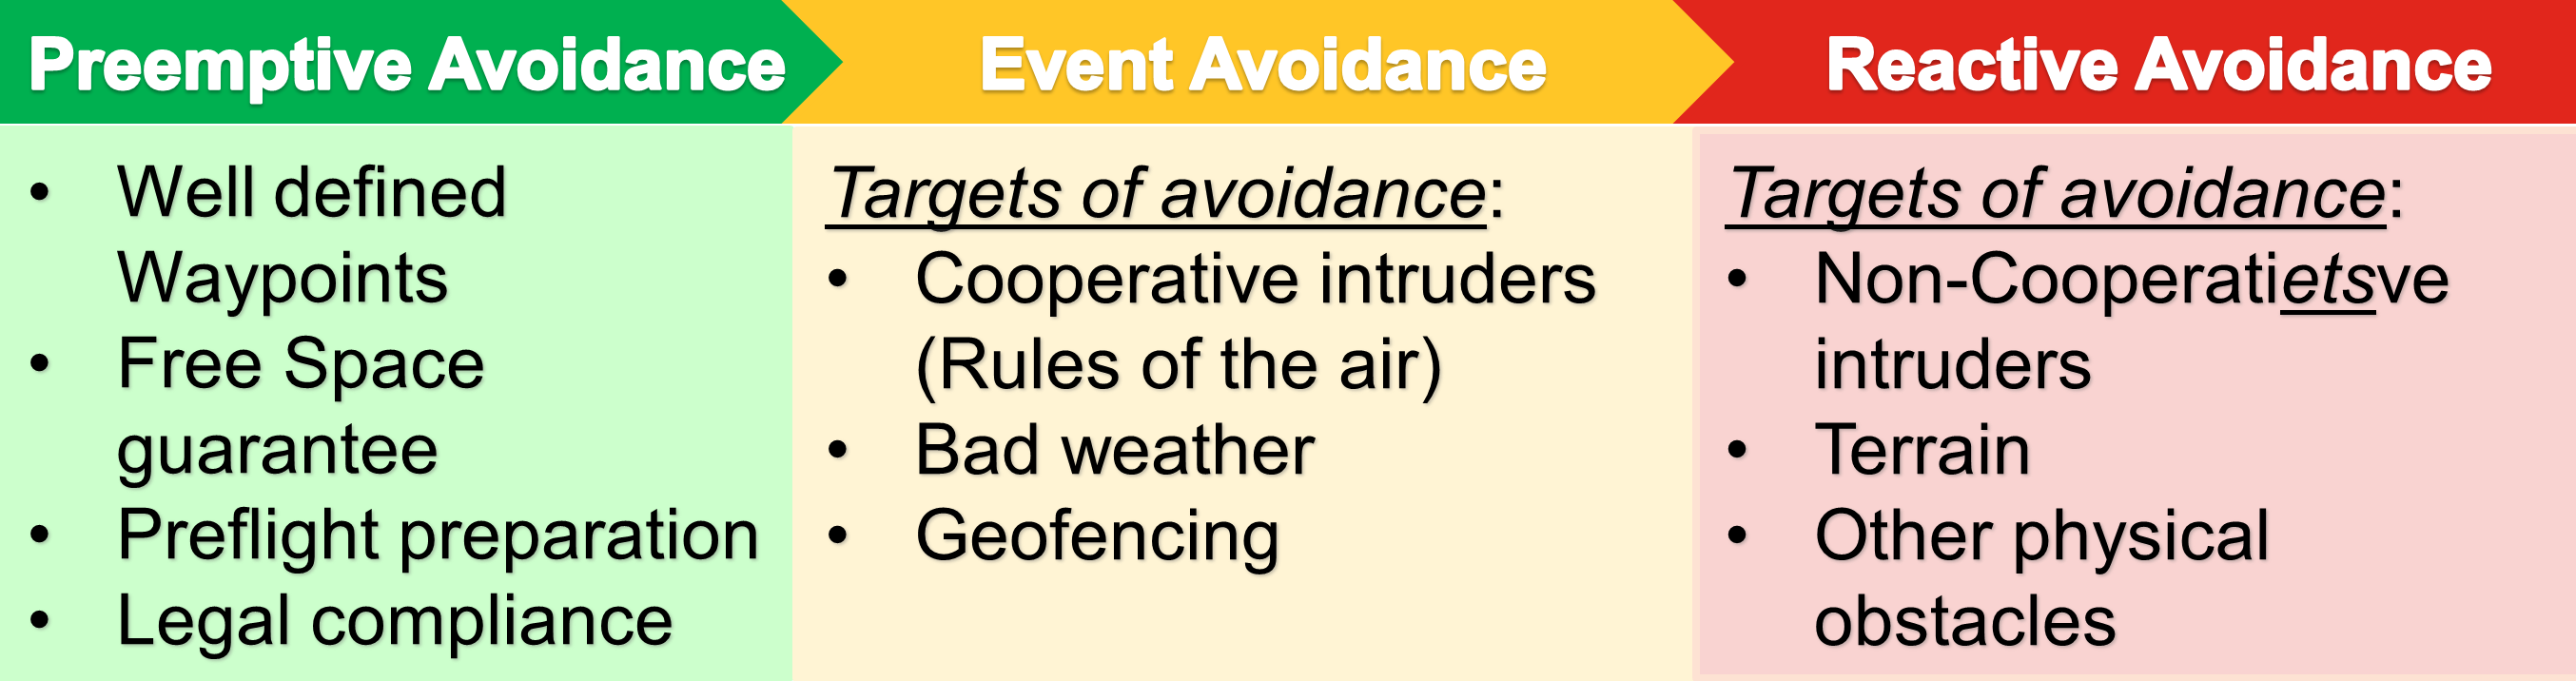
\includegraphics[width=0.7\linewidth]{\FIGDIR/RE001AvoidanceLevelsBasedOnReactionTime} 
        \caption{Avoidance levels based on reaction time.}
        \label{fig:AvoidanceLevels}
    \end{figure}